\documentclass[12pt]{article}
\usepackage[margin=1in]{geometry}
\usepackage{amsmath,amssymb,amsthm,graphicx,natbib,microtype}
\newtheorem{theorem}{Theorem}\newtheorem{corollary}[theorem]{Corollary}
\title{The Fixed-Coordinate Gauge Obstruction\\\large Identical Relative Tails with Arbitrarily Bad Loewner Transfer}
\author{Prime Dynamics Theory Program}\date{July 2026}
\begin{document}\maketitle
\begin{abstract}
We prove that the gauge in RH-120 cannot be dropped.  For every
$0<\varepsilon\leq1$ there are positive four-dimensional pairs $(G,D)$ and
$(G',D')$ with identical relative Rayleigh constants and identical
generalized spectra, related by a coordinate swap, while the best
fixed-coordinate RH-120 factor is exactly $1/\varepsilon$.  The swapping
gauge has factor one.  Thus spectral agreement of the two relative pairs
does not control a common-coordinate Loewner comparison.  A 512-point audit
from $10^{-1}$ to $10^{-14}$ has zero failures and log--log slope $-1$.
This is a sharp negative theorem, not a failure of the gauge-covariant route.
\end{abstract}

\section{Best constants without a gauge}
For $G,G',D,D'\succ0$, the largest $a$ and smallest $b$ satisfying
\[
 G'\succeq aG,\qquad D'\preceq bD
\]
are
\[
 a=\lambda_{\min}(G^{-1/2}G'G^{-1/2}),\qquad
 b=\lambda_{\max}(D^{-1/2}D'D^{-1/2}).
\]
RH-120 then gives $\gamma'\leq\sqrt{b/a}\,\gamma$.  These constants are
optimal by the variational characterization of ordered eigenvalues
\citep{Bhatia2007,HornJohnson1991}.

\section{Sharp swapped-axis obstruction}
\begin{theorem}[Unbounded fixed-coordinate loss]\label{thm:swap}
Fix $\gamma>0$ and $0<\varepsilon\leq1$.  Let
\[
 G_\varepsilon=\operatorname{diag}(\varepsilon,1,2,3),\qquad
 D_\varepsilon=\gamma^2G_\varepsilon,
\]
and let $P$ swap the first two coordinates.  Put
$G'_\varepsilon=P^*G_\varepsilon P$ and
$D'_\varepsilon=P^*D_\varepsilon P$.  Then
\[
 \gamma(G_\varepsilon,D_\varepsilon)
 =\gamma(G'_\varepsilon,D'_\varepsilon)=\gamma,
\]
but the best identity-gauge constants are $a=\varepsilon$ and
$b=\varepsilon^{-1}$.  Hence the fixed-coordinate transfer factor is
$\sqrt{b/a}=\varepsilon^{-1}$.
\end{theorem}
\begin{proof}
Both relative matrices equal $\gamma^2I$, so the Rayleigh constants agree.
The generalized eigenvalues of $(G',G)$ contain $\varepsilon$ and
$\varepsilon^{-1}$, giving $a=\varepsilon$.  Since $D'=\gamma^2G'$ and
$D=\gamma^2G$, the corresponding upper factor is $b=\varepsilon^{-1}$.
\end{proof}

\begin{corollary}[Gauge recovery]
Using $S=P$ gives $G'=S^*GS$ and $D'=S^*DS$, so RH-120 transfers with
$a=b=1$ and no loss.
\end{corollary}

The example is deliberately stronger than a mismatch of scalar norms.  The
entire generalized spectrum is unchanged.  What fails is the unproved
identification of two anisotropic frame coordinates.

\section{Audit and route consequence}
We evaluate the family at 512 logarithmically spaced anisotropies.  The
computed identity-gauge factor agrees with $1/\varepsilon$, source and target
gammas agree, and the swapping gauge has factor one in every case.  The
fitted log--log slope is $-1$ to machine precision.

\begin{figure}[h]
\centering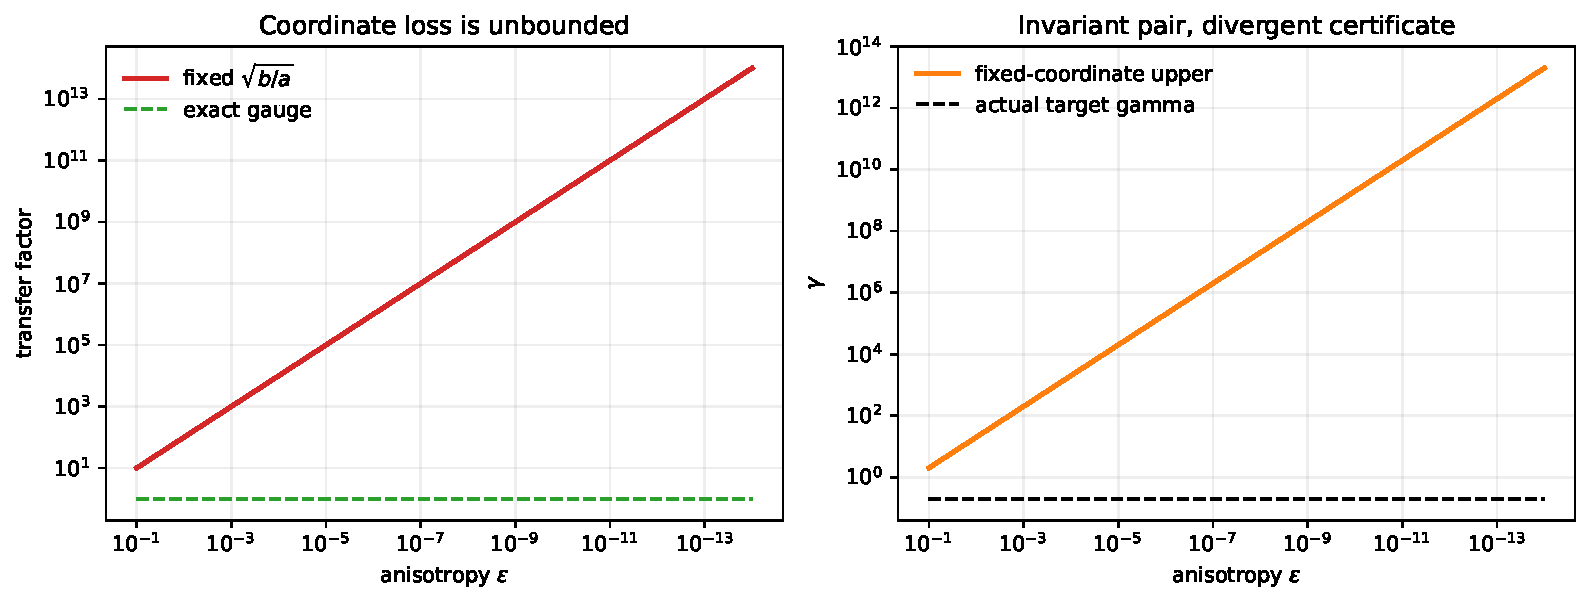
\includegraphics[width=\textwidth]{figures/fixed_coordinate_gauge_obstruction.pdf}
\caption{The physical relative pair is invariant, while a forced common
coordinate system creates an arbitrarily bad certificate.}
\end{figure}

RH-122 closes the no-gauge branch: a future cross-level proof must either
construct a gauge or prove an additional common-coordinate coherence law.
The negative result leaves the gauge-covariant route intact and motivates
the defect-stable recurrence of RH-123.  No uniform physical gauge, Stage A,
Hilbert--Polya operator, zeta-zero identification, or Riemann Hypothesis
claim is made.
\bibliographystyle{plainnat}\bibliography{references}
\end{document}
